% Created 2017-03-01 Wed 01:10
\documentclass[11pt]{article}
\usepackage[utf8]{inputenc}
\usepackage[T1]{fontenc}
\usepackage{fixltx2e}
\usepackage{graphicx}
\usepackage{longtable}
\usepackage{float}
\usepackage{wrapfig}
\usepackage{rotating}
\usepackage[normalem]{ulem}
\usepackage{amsmath}
\usepackage{textcomp}
\usepackage{marvosym}
\usepackage{wasysym}
\usepackage{amssymb}
\usepackage{hyperref}
\tolerance=1000
\usepackage[margin=0.75in]{geometry} \usepackage{graphicx}
\author{Anthony Tam, 1002583402}
\date{\today}
\title{CSC258 Prelab Six}
\hypersetup{
  pdfkeywords={},
  pdfsubject={},
  pdfcreator={Emacs 26.0.50.1 (Org mode 8.2.10)}}
\begin{document}

\maketitle


\section{States of the circuit}
\label{sec-1}
The circuit has the following states:
\begin{itemize}
\item 000 (Initial)
\item 001 (1 Click - To arm)
\item 011 (2 Clicks - To arm)
\item 010 (3 Clicks - Armed)
\item 110 (1 Click - To disarm)
\item 100 (2 Clicks - To disarm)
\item 101 (3 Clicks - Disarmed)
\end{itemize}

\section{State transition diagram}
\label{sec-2}
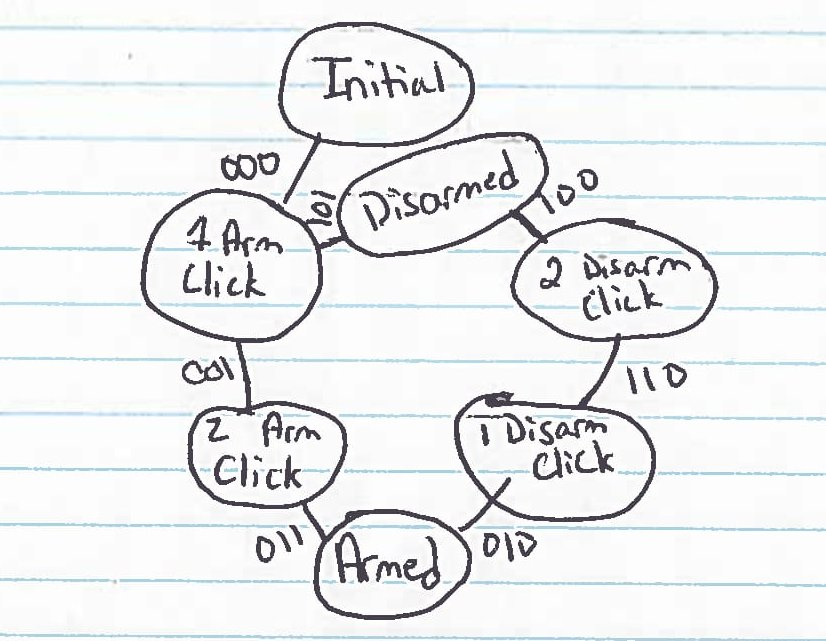
\includegraphics[width=\textwidth]{ST-1.jpg}

\section{Number of flip-flops}
\label{sec-3}
3 flip-flops are required

\section{Values of the flip-flops to avoid intermediate states}
\label{sec-4}
\begin{itemize}
\item 000
\item 001
\item 011
\item 010
\item 110
\item 100
\item 101
\end{itemize}

\section{State table}
\label{sec-5}
\begin{center}
\begin{tabular}{rrrrrrr}
F$_{\text{1}}$ & F$_{\text{2}}$ & F$_{\text{3}}$ & W & F$_{\text{1}}$ & F$_{\text{2}}$ & F$_{\text{3}}$\\
\hline
0 & 0 & 0 & 0 & 0 & 0 & 0\\
0 & 0 & 0 & 1 & 0 & 0 & 1\\
0 & 0 & 1 & 0 & 0 & 0 & 1\\
0 & 0 & 1 & 1 & 0 & 1 & 1\\
0 & 1 & 1 & 0 & 0 & 1 & 1\\
0 & 1 & 1 & 1 & 0 & 1 & 0\\
0 & 1 & 0 & 0 & 0 & 1 & 0\\
0 & 1 & 0 & 1 & 1 & 1 & 0\\
1 & 1 & 0 & 0 & 1 & 1 & 0\\
1 & 1 & 0 & 1 & 1 & 0 & 0\\
1 & 0 & 0 & 0 & 1 & 0 & 0\\
1 & 0 & 0 & 1 & 1 & 0 & 1\\
1 & 0 & 1 & 0 & 1 & 0 & 1\\
1 & 0 & 1 & 1 & 0 & 0 & 1\\
\end{tabular}
\end{center}

\section{Combinational Logic}
\label{sec-6}
F$_{\text{1}}$: F$_{\text{1}}$$\cdot$$\overline{F_{3}}$ + F$_{\text{1}}$$\cdot$$\overline{W}$ + W$\cdot$F$_{\text{0}}$$\cdot$\overline{F_3}\\
F$_{\text{2}}$: \overline{F_1}$\cdot$F$_{\text{3}}$$\cdot$W + \overline{F_1}$\cdot$F$_{\text{2}}$ + F$_{\text{2}}$$\cdot$\$\overline{W}\$\\
F$_{\text{3}}$: F$_{\text{3}}$$\cdot$\overline{W} + \overline{F_2}$\cdot$W

\section{Flip-flop circuit diagram}
\label{sec-7}
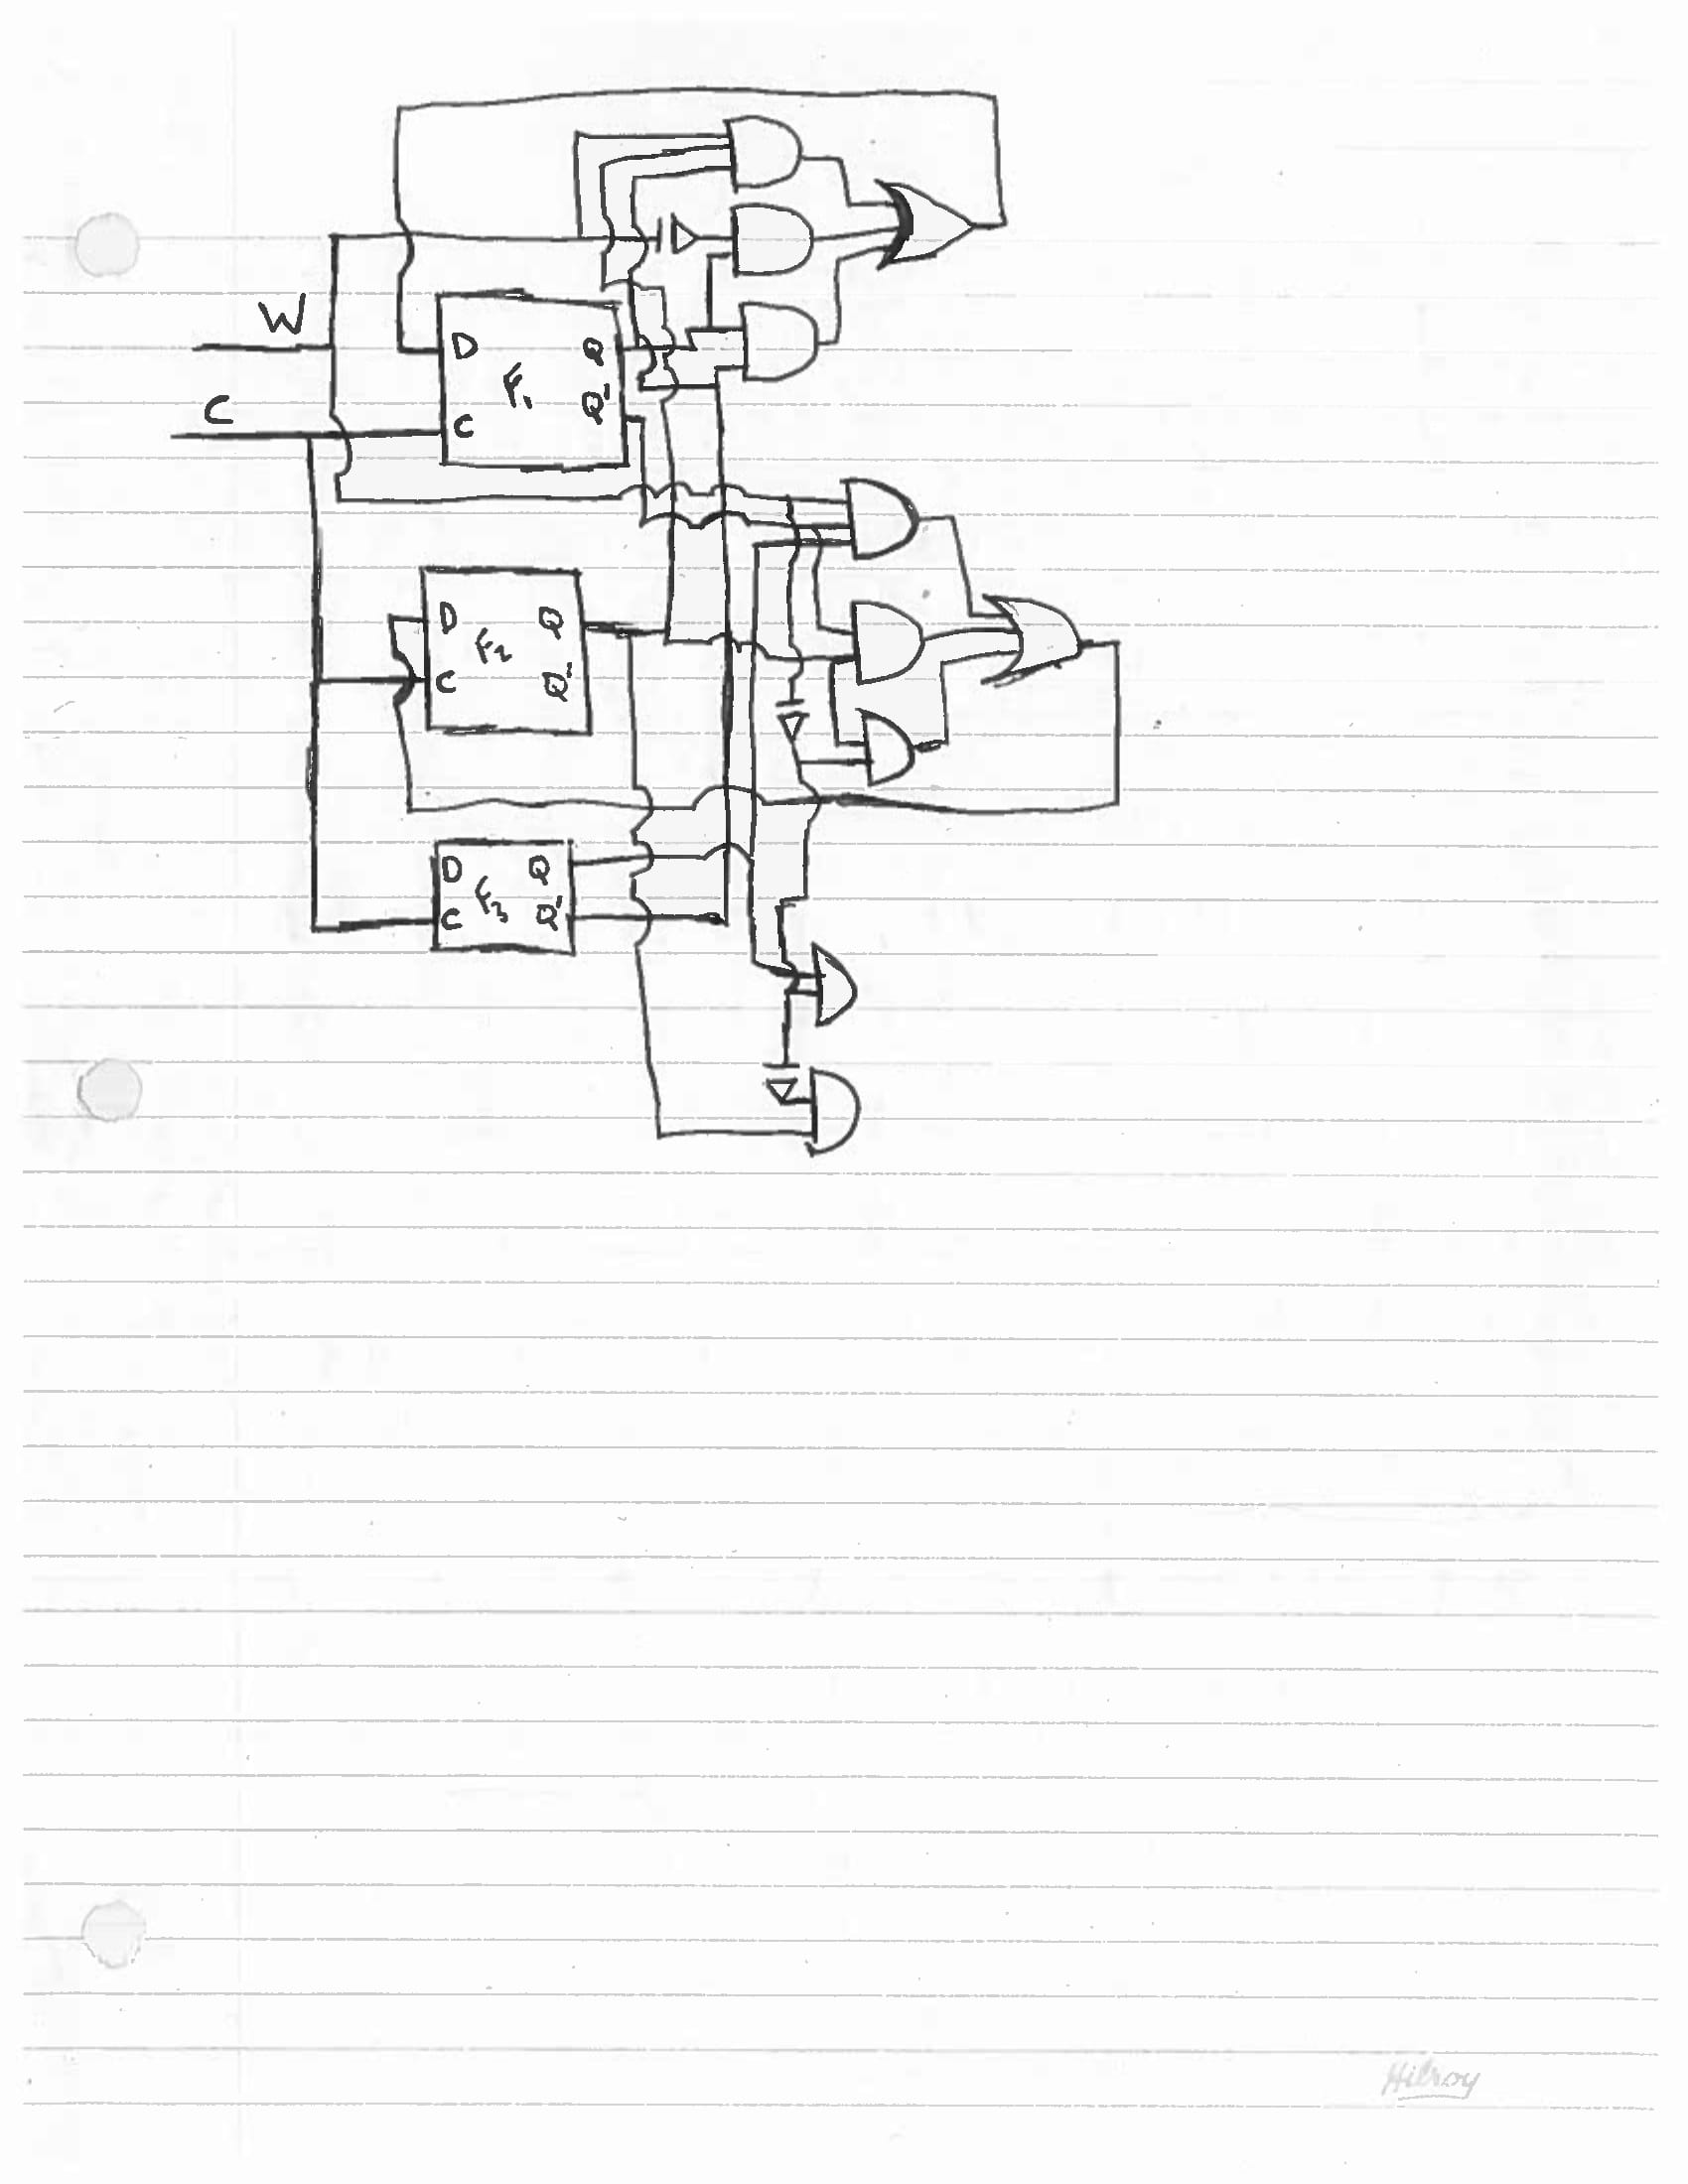
\includegraphics[width=\textwidth]{CD1-1.jpg}

\section{State Values}
\label{sec-8}
\begin{itemize}
\item State 010 is the armed state
\item State 101 is the disarmed state
\end{itemize}

\section{Output logic statements}
\label{sec-9}
Armed: \overline{F_1}$\cdot$F$_{\text{2}}$$\cdot$\overline{F_3}\\
Disarmed: F$_{\text{1}}$$\cdot$\overline{F_2}$\cdot$F$_{\text{3}}$

\section{Modified circuit diagram}
\label{sec-10}
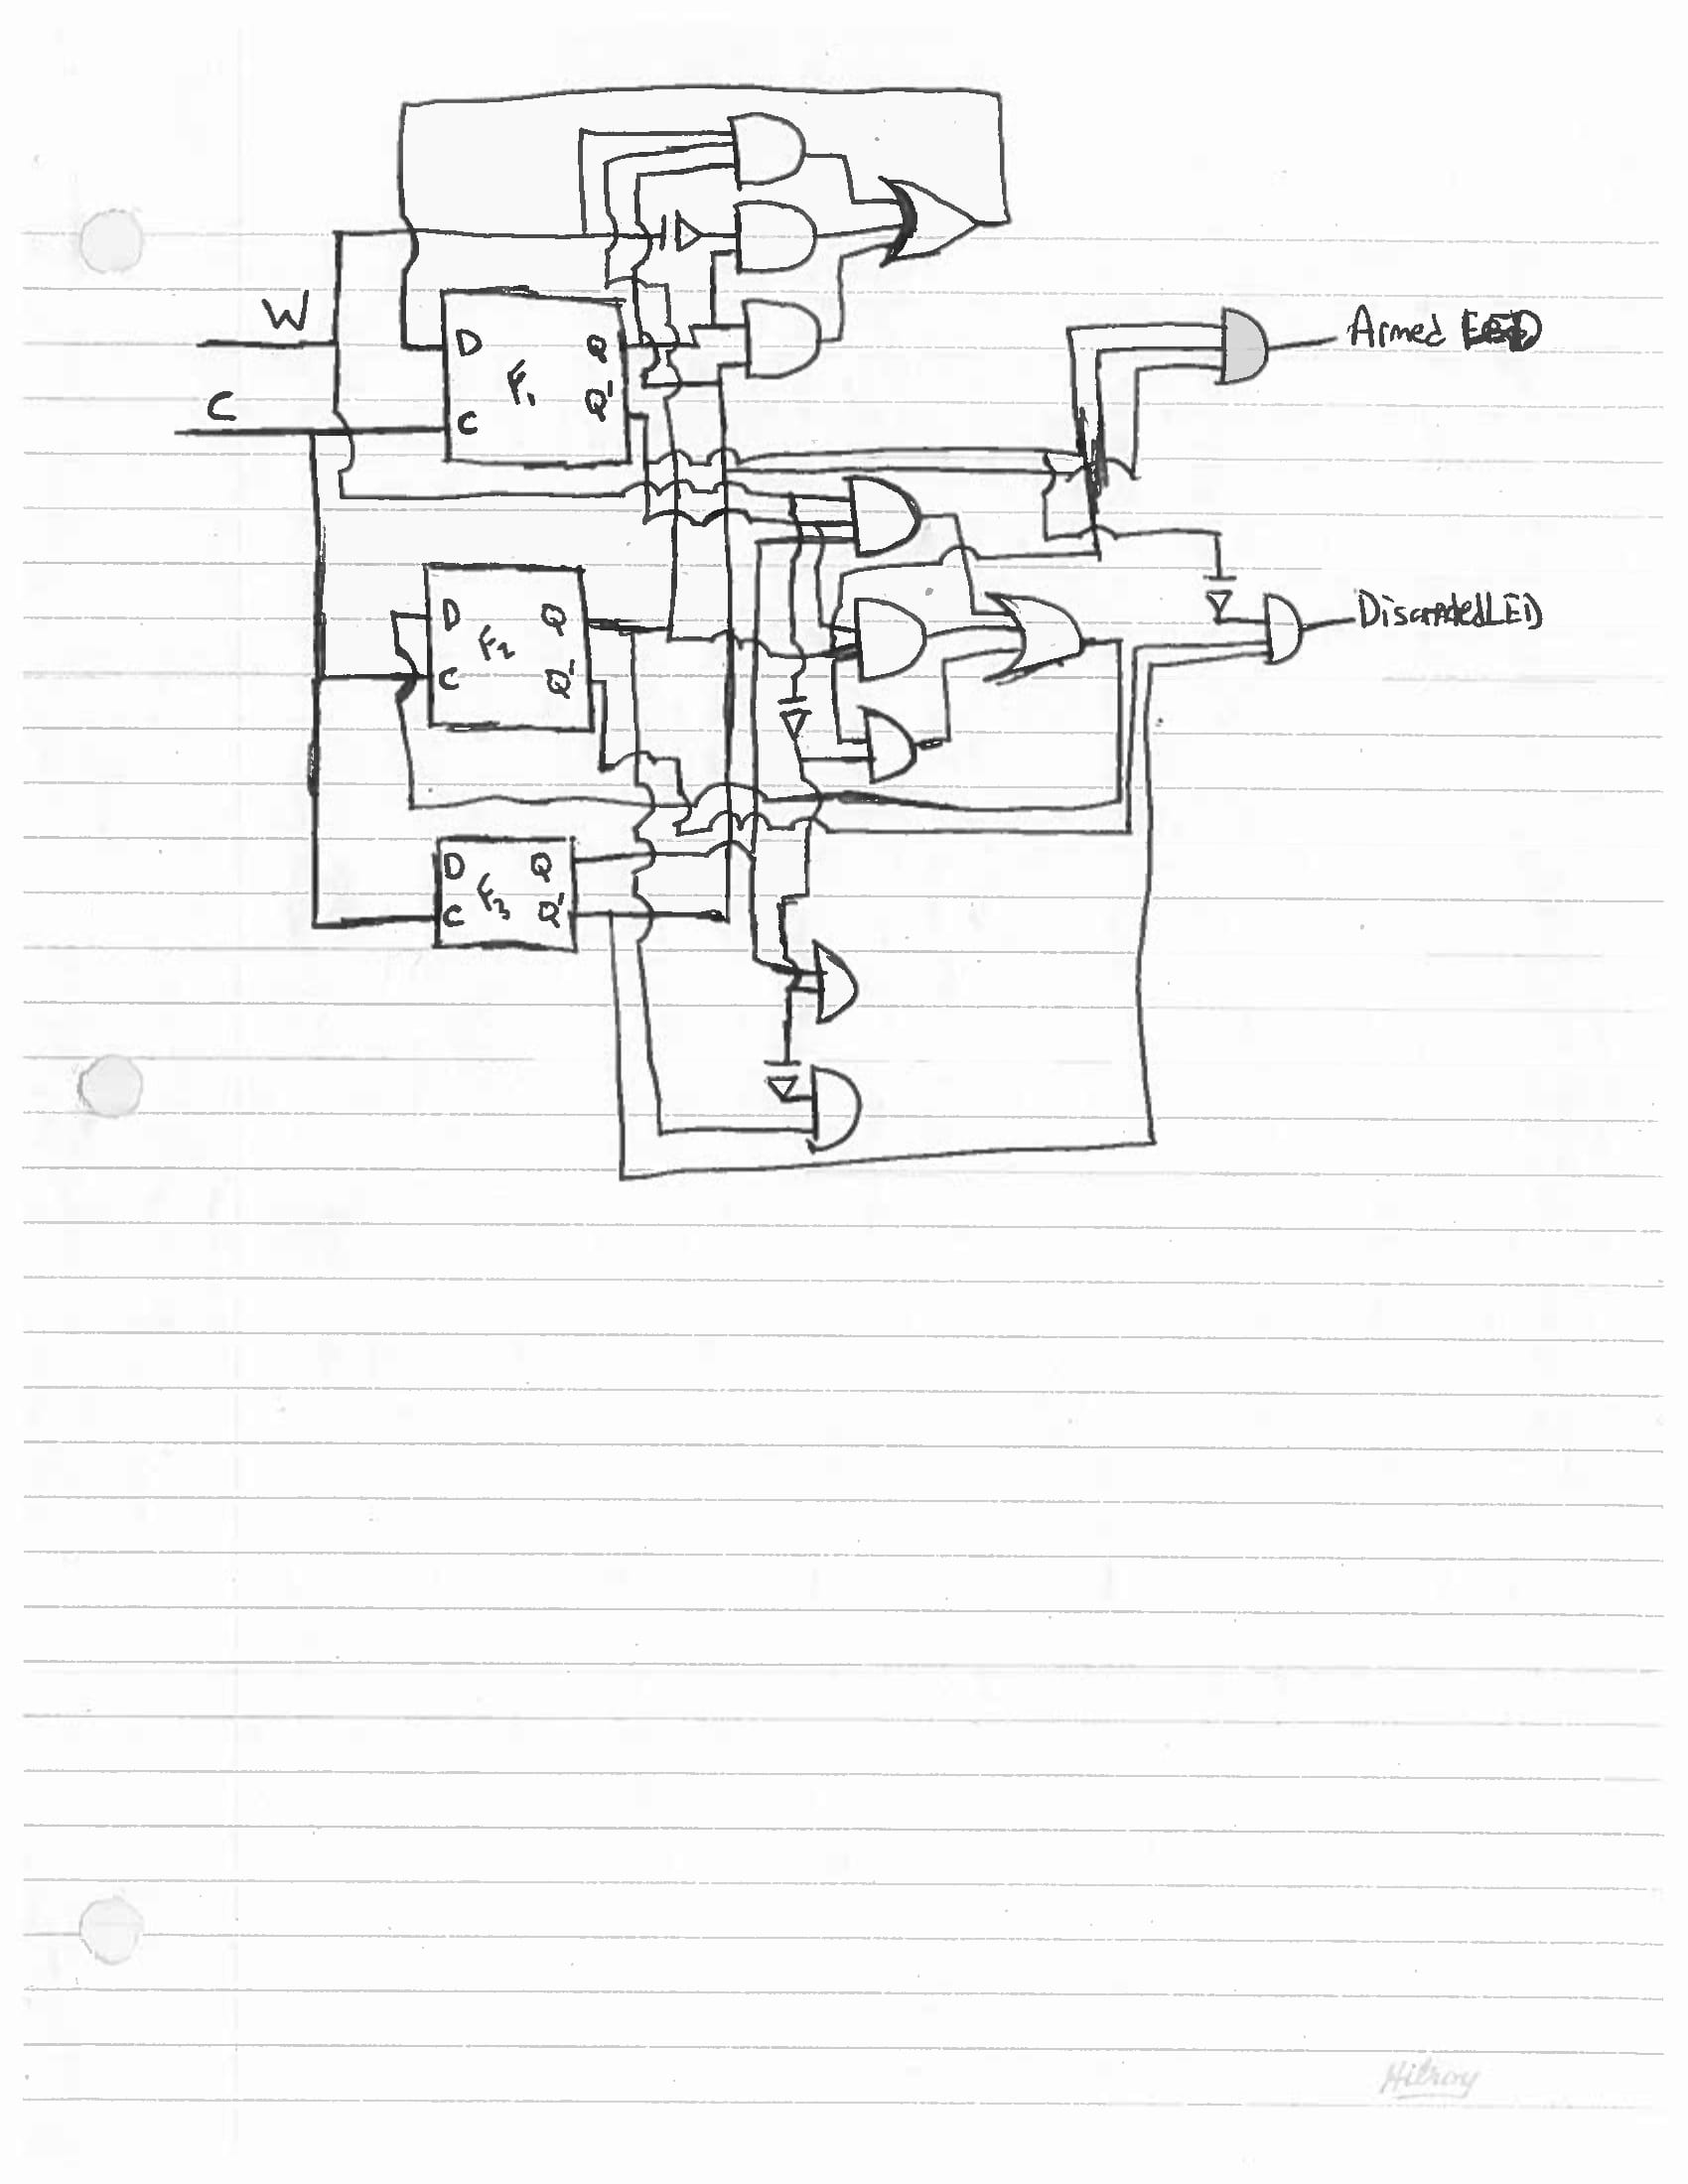
\includegraphics[width=\textwidth]{CD2-1.jpg}
% Emacs 26.0.50.1 (Org mode 8.2.10)
\end{document}
